\subsubsection{Action Generation Evaluation}
\label{subsec::action_benchmarks}

We evaluate whether action mid-training endows Cosmos 3 with a reusable world-action prior across domains and inference modes.
The central question is whether unified action mid-training accelerates adaptation to a domain-specific action interface, and whether a short post-training stage can turn the shared base model into a specialized model that is competitive with or stronger than state-of-the-art domain baselines.
\Cref{tab:action_posttraining_summary_wide} reports results on camera motion, autonomous driving, robotics, and egocentric motion domains, covering forward- and inverse-dynamics settings.
\Cref{tab:action_posttraining_policy} reports results on robot policy settings, evaluating Cosmos 3's ability to complete language-specified tasks.

\paragraph{Setup.} We compare two initialization protocols for each downstream domain. The first, pre-training initialization (\textit{PT-init}), starts from the Cosmos 3 pre-trained checkpoint, which has not been trained on action-domain data. The second, mid-training initialization (\textit{MT-init}), starts from our mid-trained checkpoint, which has seen action data spanning multiple domains and prediction modes, including forward dynamics (FD), inverse dynamics (ID), and policy. For each comparison, we use the same training recipe and keep the model size, data, and compute budget fixed. We report results for both Cosmos3-Nano and Cosmos3-Super.

\paragraph{Metrics.} We report metrics for each action interface. For autonomous-vehicle inverse dynamics, relative rotation error (RRE) and relative translation error (RTE) measure frame-to-frame pose accuracy, while absolute trajectory error (ATE) measures global trajectory consistency. We also use these metrics to measure camera-following accuracy in camera-motion forward dynamics, comparing the ground-truth camera poses with the estimated camera trajectories from generated videos. For robotics and egocentric forward dynamics, PSNR measures the reconstruction quality of action-conditioned future observations. Although a plausible generative rollout need not be pixel-identical to the single recorded ground-truth future, we find that PSNR is as a useful proxy for temporal alignment, motion consistency, and reconstruction fidelity under a relatively short temporal horizon. For robotics policy, success rate measures the percentage of evaluation tasks completed successfully.

\begin{table}[t]
    \centering
    \caption{\textbf{Post-training comparisons for forward and inverse dynamics across domains.} FD denotes forward dynamics and ID denotes
  inverse dynamics. \textit{PT-init} initializes from the generic Cosmos 3 pre-trained checkpoint, while \textit{MT-init} initializes from
  the mid-trained checkpoint. Domain-specific baselines are reported only for their corresponding application, while Cosmos 3 variants are compared across all evaluated action settings. \textbf{Bold} indicates the best in the column and
  \underline{underline} indicates the second best.}
  \label{tab:action_posttraining_summary_wide}
    \small
    \setlength{\tabcolsep}{5pt}
    \resizebox{\linewidth}{!}{%
    \begin{tabular}{@{}l|ccc|ccc|c|c@{}}
        \toprule
        & \multicolumn{3}{c|}{\textbf{Autonomous Vehicle (ID)}} & \multicolumn{3}{c|}{\textbf{Camera Motion (FD)}} & \multicolumn{1}{c|}{\textbf{Egocentric Motion (FD)}} & \textbf{Robotics (FD)} \\
        \cmidrule(lr){2-4} \cmidrule(lr){5-7} \cmidrule(lr){8-8} \cmidrule(lr){9-9}
        \textbf{Model} & RRE ($^\circ$, $\downarrow$) & RTE (m, $\downarrow$) & ATE (m, $\downarrow$) & RRE ($^\circ$, $\downarrow$) & RTE (m, $\downarrow$) & ATE (m, $\downarrow$) & PSNR ($\uparrow$) & PSNR ($\uparrow$) \\
        \midrule
        \rowcolor{rowours}
        \textbf{Cosmos3-Super} (\textit{MT-init}) & \underline{0.232} & \textbf{0.014} & \textbf{0.90} & \textbf{0.142} & \textbf{0.026} & \textbf{0.99} & \textbf{16.19} & \textbf{26.04} \\
        \rowcolor{rowours}
        \textbf{Cosmos3-Nano} (\textit{MT-init})  & \textbf{0.211} & \textbf{0.014} & \underline{0.98} & \underline{0.147} & \underline{0.029} & \underline{1.24} & \underline{16.12} & \underline{25.52} \\
        \midrule
        \rowcolor{rowours}
        \textbf{Cosmos3-Super} (\textit{PT-init}) & 0.284 & 0.018 & 1.32 & 0.293 & 0.036 & 1.82 & 15.34 & 22.69 \\
        \rowcolor{rowours}
        \textbf{Cosmos3-Nano} (\textit{PT-init})  & 0.249 & \underline{0.017} & 1.20 & 0.172 & 0.034 & 1.61 & 15.22 & 23.24 \\
        \midrule
        Lingbot-World  & --    & --    & --    & 0.299 & 0.057 & 2.88 & --    & --    \\
        HY-World1.5 & --    & --    & --    & 0.377 & 0.042 & 1.39 & --    & --    \\
        \midrule
        VGGT           & 0.596 & 0.768 & 23.46 & --    & --    & --   & --    & --    \\
        DepthAnything3 & 0.312 & 0.354 & 9.29  & --    & --    & --   & --    & --    \\
        \midrule
        LOME       & -- & -- & -- & -- & -- & -- & 9.36 & --    \\
        \midrule
        Ctrl-World & -- & -- & -- & -- & -- & -- & --   & 22.99 \\
        \bottomrule
    \end{tabular}
    }
\end{table}

\paragraph{Autonomous vehicle (ID).} 
We evaluate the inverse-dynamics capabilities of Cosmos 3 using an in-house driving dataset, which consists of 6-second video clips with accurate ego-vehicle trajectories at 10 FPS. 
Under this setup, the model directly predicts the ego-trajectory from video inputs. 
We compare our approach against two state-of-the-art general-domain baselines: VGGT~\citep{wang2025vggt} and DepthAnything3~\citep{lin2025depthanything3}. 
As reported in~\cref{tab:action_posttraining_summary_wide}, both Cosmos3-Nano and Cosmos3-Super initialized with \textit{PT-init} outperform the baselines. 
Applying \textit{MT-init} yields further improvements for Cosmos3-Nano. 
Notably, our method trained with specialized driving data achieves much better metric-scale translation estimation, whereas the general-domain baselines suffer from drifting errors. 
Overall, these results demonstrate that physical-AI-oriented video models can excel in specific embodied applications with minimal adaptation. 
Qualitative results are visualized in~\cref{fig:av_id}.

\begin{figure}[t]
    \centering
    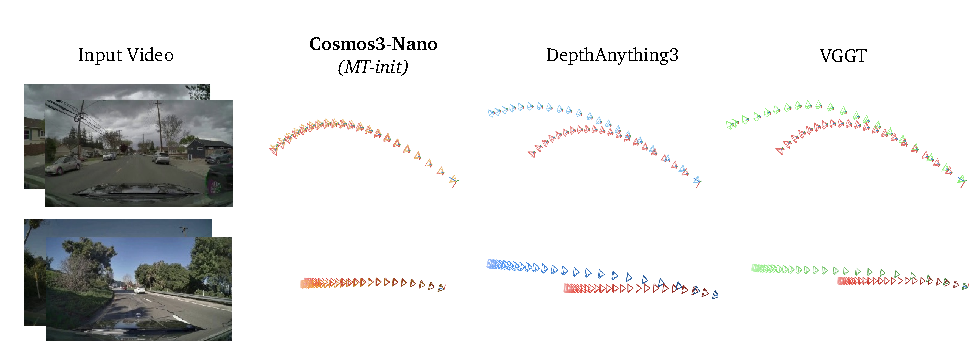
\includegraphics[width=0.99007\linewidth]{figures/results/action/av_id_figure.pdf}
    \caption{\textbf{Comparison for autonomous vehicle inverse dynamics}. We qualitatively compare ego-vehicle trajectories estimated from input videos by different methods, with the red trajectory representing the ground truth. \textbf{Cosmos3-Nano} \textit{(MT-init)} demonstrates the ability to estimate accurate, metric-scale ego poses.}
    \label{fig:av_id}
\end{figure}


\paragraph{Camera motion (FD).}
\label{sec:camera_fdm}
Camera-conditioned video generation can serves as world simulation for many applications. 
We task the model with predicting future frames given an initial image and a specified camera trajectory.
To quantify camera-following accuracy, we utilize DepthAnything3~\citep{lin2025depthanything3} to estimate metric-scale camera trajectories from the generated videos and compare them against the conditioning input.
If the generated videos are highly consistent with the conditioning trajectory, the estimated poses from the predicted sequence should closely match the input poses.
We benchmark our approach against the bidirectional models of Lingbot-World~\citep{lingbot-world} and HY-World 1.5~\citep{hyworld2025} on an internal dataset of one hundred 5-second realistic video clips with camera motions estimated by DepthAnything3~\citep{lin2025depthanything3}. Qualitative results are reported in~\cref{fig:camera_fd}. 
The results show that Cosmos3-Nano and Cosmos3-Super with \textit{PT-init} already provide robust camera control. 
\textit{MT-init} improves the result further: Cosmos3-Super achieves 0.142$^\circ$ RRE, 0.026 m RTE, and 0.99 m ATE, outperforming Lingbot-World (0.299$^\circ$ RRE, 0.057 m RTE, 2.88 m ATE) and HY-World 1.5 (0.377$^\circ$ RRE, 0.042 m RTE, 1.39 m ATE) across all three metrics.

\begin{figure}[hbt]
    \centering
    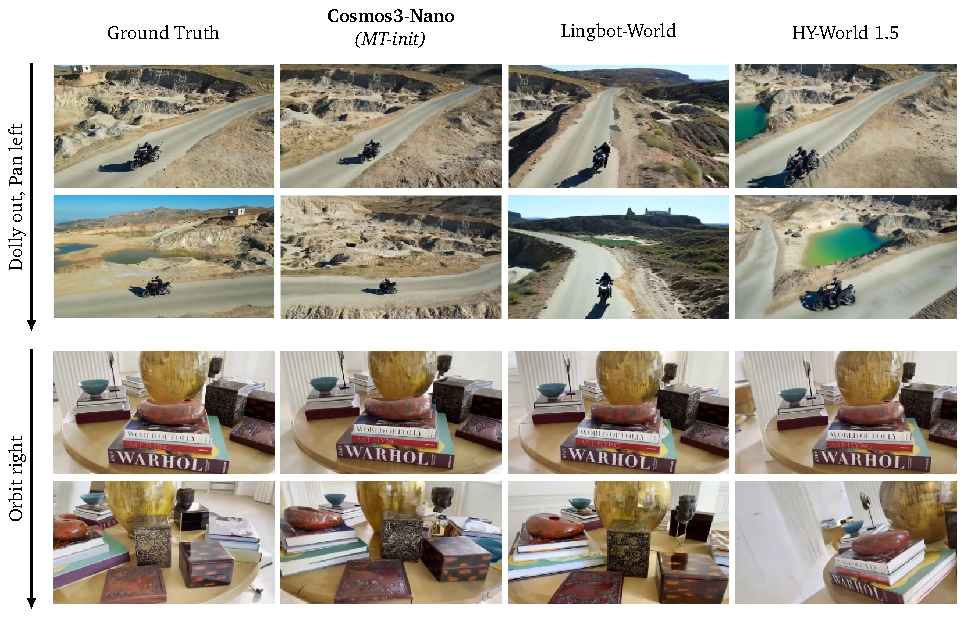
\includegraphics[width=0.98415\linewidth]{figures/results/action/camera_fd_figure.pdf}
    \caption{\textbf{Camera forward dynamics comparison}. Given complex realistic trajectories, \textbf{Cosmos3-Nano} \textit{(MT-init)} faithfully reproduces the same camera motion in the generated video. For each motion example, the first row shows frames near the start of the sequence and the second row shows frames near the end. The downward arrow indicates temporal progression from start to finish, while the text beside it specifies the commanded camera motion.}
    \label{fig:camera_fd}
\end{figure}


\paragraph{Egocentric motion (FD).}
\label{sec:egocentric_fdm}
We evaluate videos from Human World Bench (HWB, see \cref{subsec::hwb}) in the forward-dynamics
setting. We use the HWB action annotations, which include both camera ego-motion and hand motion tracking, and report the PSNR of the generated
videos. We adapt both \textit{PT-init} and \textit{MT-init} checkpoints to the egocentric domain and compare against LOME~\citep{gao2026lome}, a recent action-conditioned video generation method specialized for egocentric hand manipulation data. 
Although LOME is one of the closest available baselines for this setting, it performs poorly on HWB, achieving a PSNR value of 9.36dB, likely due to distribution shift between its training data and the HWB benchmark.
In contrast, Cosmos 3 achieves substantially higher PSNR across both model scales and initialization protocols. With \textit{PT-init},
Cosmos3-Nano reaches a PSNR value of 15.22dB and Cosmos3-Super reaches a PSNR value of 15.34dB. 
Starting from \textit{MT-init}
further improves the scores to PSNR values of 16.12dB for Cosmos3-Nano and 16.19dB for Cosmos3-Super. 
These results show that \textit{MT-init} provides a consistent gain, indicating that unified action mid-training
provides a substantially stronger starting point for egocentric forward dynamics.
Overall, these results support the central hypothesis of unified action mid-training: co-training across robot embodiments, camera
motion, autonomous-vehicle motion, and egocentric motion induces a transferable action-domain prior, enabling faster convergence and
stronger downstream adaptation in the egocentric domain.

\paragraph{Robotics (FD).}
\label{sec:robot_fdm}
Robotics forward dynamics unlocks applications such as policy evaluations with video models.
We conduct experiments on the DROID dataset~\citep{khazatsky2024droid}, a large-scale real-robot manipulation dataset featuring diverse scenes and objects. 
Given an initial frame and the robot end-effector action chunk of size 16, the model predicts the subsequent 16 frames.
We post-train both the \textit{PT-init} and \textit{MT-init} checkpoints on the DROID dataset.
We compare against Ctrl-World~\citep{guo2026ctrlworld} as our primary baseline.
We present the qualitative results in \cref{fig:robotics_fd_qualitative} and quantitative results in~\cref{tab:action_posttraining_summary_wide}.
As shown in \cref{tab:action_posttraining_summary_wide}, post-training from the pre-trained checkpoint already matches the baseline at Nano scale, reaching a PSNR value of 23.24dB compared with 22.99dB for Ctrl-World. 
Post-training from the mid-trained checkpoint yields substantially stronger results, reaching PSNR values of 25.52dB with Cosmos3-Nano and 26.04dB with Cosmos3-Super. 
These results demonstrate that Cosmos 3 is a strong and flexible backbone for forward dynamics prediction.
\begin{figure*}[t]
    \centering
    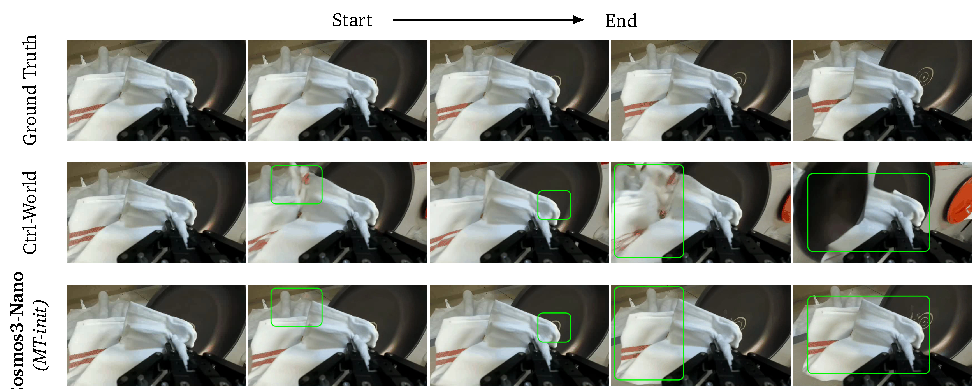
\includegraphics[width=0.98810\linewidth]{figures/results/action/robotics_fd_figure.pdf}
    \caption{\textbf{Qualitative comparison for robotics forward dynamics.} The generated frames closely follow the action commands, and the interactions between the robot arm and the fabric are more realistic than those from the baseline. Green boxes highlight regions with visible distortions or artifacts in the baseline outputs, and the corresponding regions in \textbf{Cosmos3-Nano} \textit{(MT-init)}, where these artifacts are absent.}
    \label{fig:robotics_fd_qualitative}
\end{figure*}


\paragraph{Robot manipulation (policy).}
\label{sec:robot_manip_policy}
To evaluate the policy mode, we post-train and submit our Cosmos3-Nano-Policy-DROID to the RoboLab simulation benchmark~\citep{yang2026robolab} and the RoboArena real-world benchmark~\citep{atreya2025roboarena}. 
As shown in~\cref{tab:action_posttraining_policy} and~\cref{fig:robotarena_leaderboard}, our model achieves new state-of-the-art results on both benchmarks, demonstrating that our Cosmos3 omnimodal world models can be further post-trained into strong robot manipulation policy models.

RoboLab~\citep{yang2026robolab} is a high-fidelity, robot- and policy-agnostic simulation benchmark comprising 120 language-conditioned tasks designed to evaluate task-generalist robot manipulation policies across visual, relational, and procedural competencies.
RoboLab evaluates each task under three instruction specificity levels, across vague prompts, default prompts and specific prompts.
This split tests robustness to language phrasing rather than a single canonical command.
On RoboLab, our post-trained policy surpasses all prior models on task success rate by clear margins (\cref{tab:action_posttraining_policy}), including strong vision-language-action (VLA) models such as $\pi_{0.5}$~\citep{pi05} and world-action models (WAM) such as DreamZero~\citep{ye2026dreamzero},
across all task instruction granularities and task difficulty levels.
For example, under \textit{specific} task instructions, our policy achieves a 39.7\% average success rate across 120 tasks with 10 rollouts per task, outperforming $\pi_{0.5}$ at 28.1\% and DreamZero at 25.2\%.
Additionally, compared with a model post-trained directly from the pre-trained checkpoint, Cosmos3-Nano (\textit{PT-init}), our final policy performs better, demonstrating the effectiveness of incorporating action-modality data from diverse sources into mid-training.

\begin{table}[t]
    \centering
    \caption{\textbf{Cosmos3-Nano-Policy-DROID establishes a new state of the art on RoboLab.}
    Task success rates (\%) are reported on RoboLab-120 across language specificity levels and task difficulty levels.
    All policies use off-the-shelf checkpoints fine-tuned on the DROID dataset.
    \textbf{Bold} indicates the best in the column.}
    \label{tab:action_posttraining_policy}
    \small
    \setlength{\tabcolsep}{4pt}
    \resizebox{\linewidth}{!}{%
    \begin{tabular}{@{}l|ccc|ccc|ccc|ccc@{}}
        \toprule
        & \multicolumn{3}{c}{\textbf{Overall}} & \multicolumn{3}{c}{\textbf{Simple}} & \multicolumn{3}{c}{\textbf{Moderate}} & \multicolumn{3}{c}{\textbf{Complex}} \\
        \cmidrule(lr){2-4} \cmidrule(lr){5-7} \cmidrule(lr){8-10} \cmidrule(lr){11-13}
        \textbf{Model} & Vague & Default & Specific & Vague & Default & Specific & Vague & Default & Specific & Vague & Default & Specific \\
        \midrule
        \rowcolor{rowours}
        \textbf{Cosmos3-Nano-Policy-DROID} & \textbf{20.6} & \textbf{36.8} & \textbf{39.7} & \textbf{23.3} & \textbf{40.6} & \textbf{42.0} & \textbf{23.3} & \textbf{35.4} & \textbf{40.3} & 4.1  & \textbf{25.3} & \textbf{29.4} \\
        \rowcolor{rowours}
        \textbf{Cosmos3-Nano} (\textit{PT-init})  & 16.7 & 28.1 & 30.2 & 17.8 & 30.3 & 32.8 & 19.0 & 28.7 & 29.5 & \textbf{7.1} & 18.2 & 21.8 \\
        \midrule
        $\pi_{0.5}$       &  15.2 &  28.0 &  28.1 &  16.2 &  29.7 &  29.8 &  17.9 &  31.5 &  31.0 & 5.3 &  13.5 &  14.7 \\
        DreamZero         &  14.9 &  25.7 &  23.9 &  15.0 &  26.1 &  25.8 &  19.5 &  30.0 &  26.7 & 4.1 &  14.1 &  10.6 \\
        $\pi_{0}$-FAST    & ~~9.2 &  15.5 &  14.9 & ~~9.5 &  20.2 &  19.4 &  12.8 &  13.3 &  12.6 & 0.0 & ~~2.9 & ~~3.5 \\
        paligemma-binning & ~~3.1 & ~~3.4 & ~~5.5 & ~~2.2 & ~~3.4 & ~~4.1 & ~~5.9 & ~~4.9 &  10.3 & 0.0 & ~~0.0 & ~~0.0 \\
        GR00T N1.6        & ~~5.4 & ~~7.2 & ~~5.3 & ~~7.2 & ~~8.8 & ~~7.5 & ~~4.9 & ~~7.9 & ~~4.1 & 0.0 & ~~0.0 & ~~0.0 \\
        $\pi_{0}$         & ~~2.8 & ~~5.0 & ~~3.5 & ~~2.8 & ~~7.2 & ~~5.3 & ~~3.8 & ~~3.6 & ~~2.1 & 0.0 & ~~0.0 & ~~0.0 \\
        \bottomrule
    \end{tabular}
    }
\end{table}
\begin{figure}[ht]
    \centering
    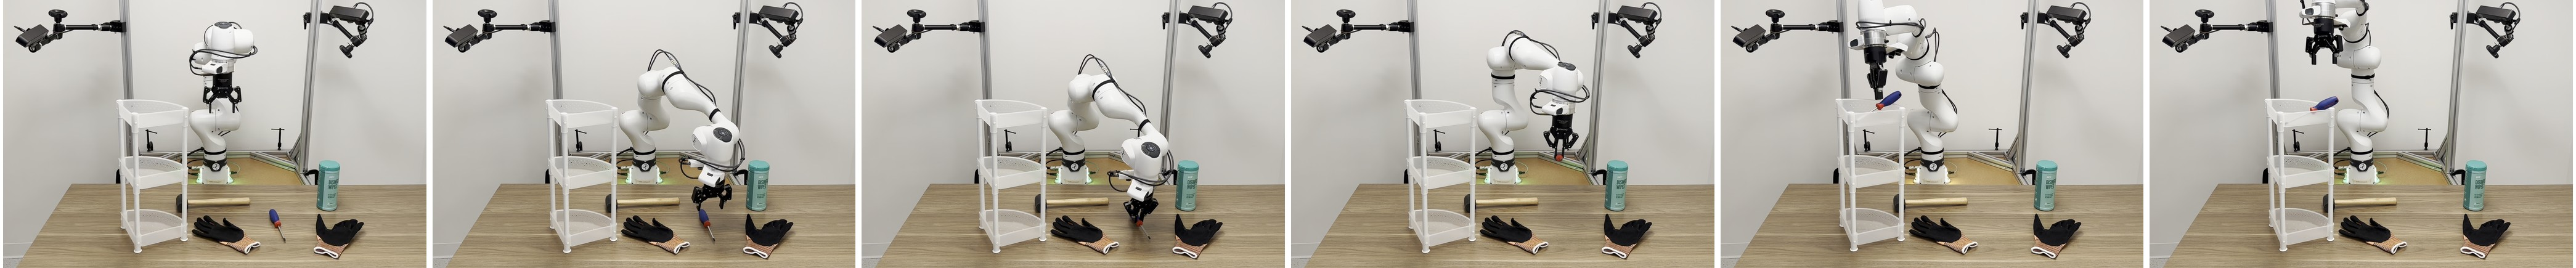
\includegraphics[width=0.99\linewidth]{figures/results/action/snapshots_20260520_02_put_the_screwdriver_on_the_top_shelf_view_1_zoom_tlr10_spaced.jpg}
    {\small Task: put the screwdriver on the top shelf\par}
    \vspace{4pt}
    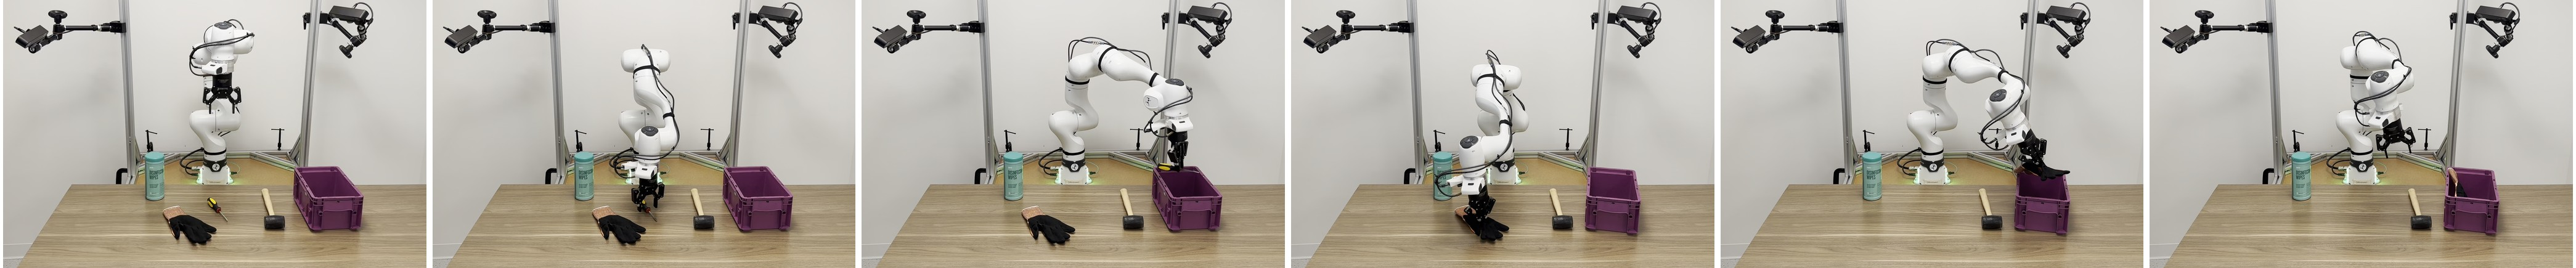
\includegraphics[width=0.99\linewidth]{figures/results/action/snapshots_20260520_01_put_the_screwdriver_and_the_glove_in_the_purple_container_view_1_zoom_tlr10_spaced.jpg}
    {\small Task: put the screwdriver and the glove in the purple container\par}
    \caption{\textbf{Real-world evaluation of Cosmos3-Nano-Policy-DROID.} We show snapshot frames from physical-robot rollouts. These examples demonstrate successful real-world deployment of our policy for language-conditioned manipulation tasks on physical robots.}
    \label{fig:robot_policy_example}
\end{figure}


RoboArena~\citep{atreya2025roboarena} is a distributed, real-world benchmark that uses crowdsourced pairwise comparisons to evaluate and rank generalist robot policies across diverse tasks and real world environments.
Anyone with a DROID platform can evaluate a pair of policies in any environment and on any task by conducting double-blind A/B comparisons, and the final scores are aggregated from these pairwise preferences to produce an overall rating for each policy.
As of 2:40 p.m. on May 30, 2026, our robot manipulation policy tops the leaderboard (\cref{fig:robotarena_leaderboard}), outperforming many prior strong policy models. 
We expect to receive more evaluations from the community, which will further validate our policy. 
Across several tested tasks, the policy accomplishes tasks reliably and follows language instructions well.
The policy can perform simple pick-and-place tasks, as well as long-horizon tasks requiring multiple sequential steps.
We observe strong generalization to a variety of unseen objects and tasks.
The policy also tolerates failures, often retrying when necessary, and remains robust to human interventions during execution.
Some qualitative results are shown in~\cref{fig:robot_policy_example}.


\begin{figure}[t]
    \centering
    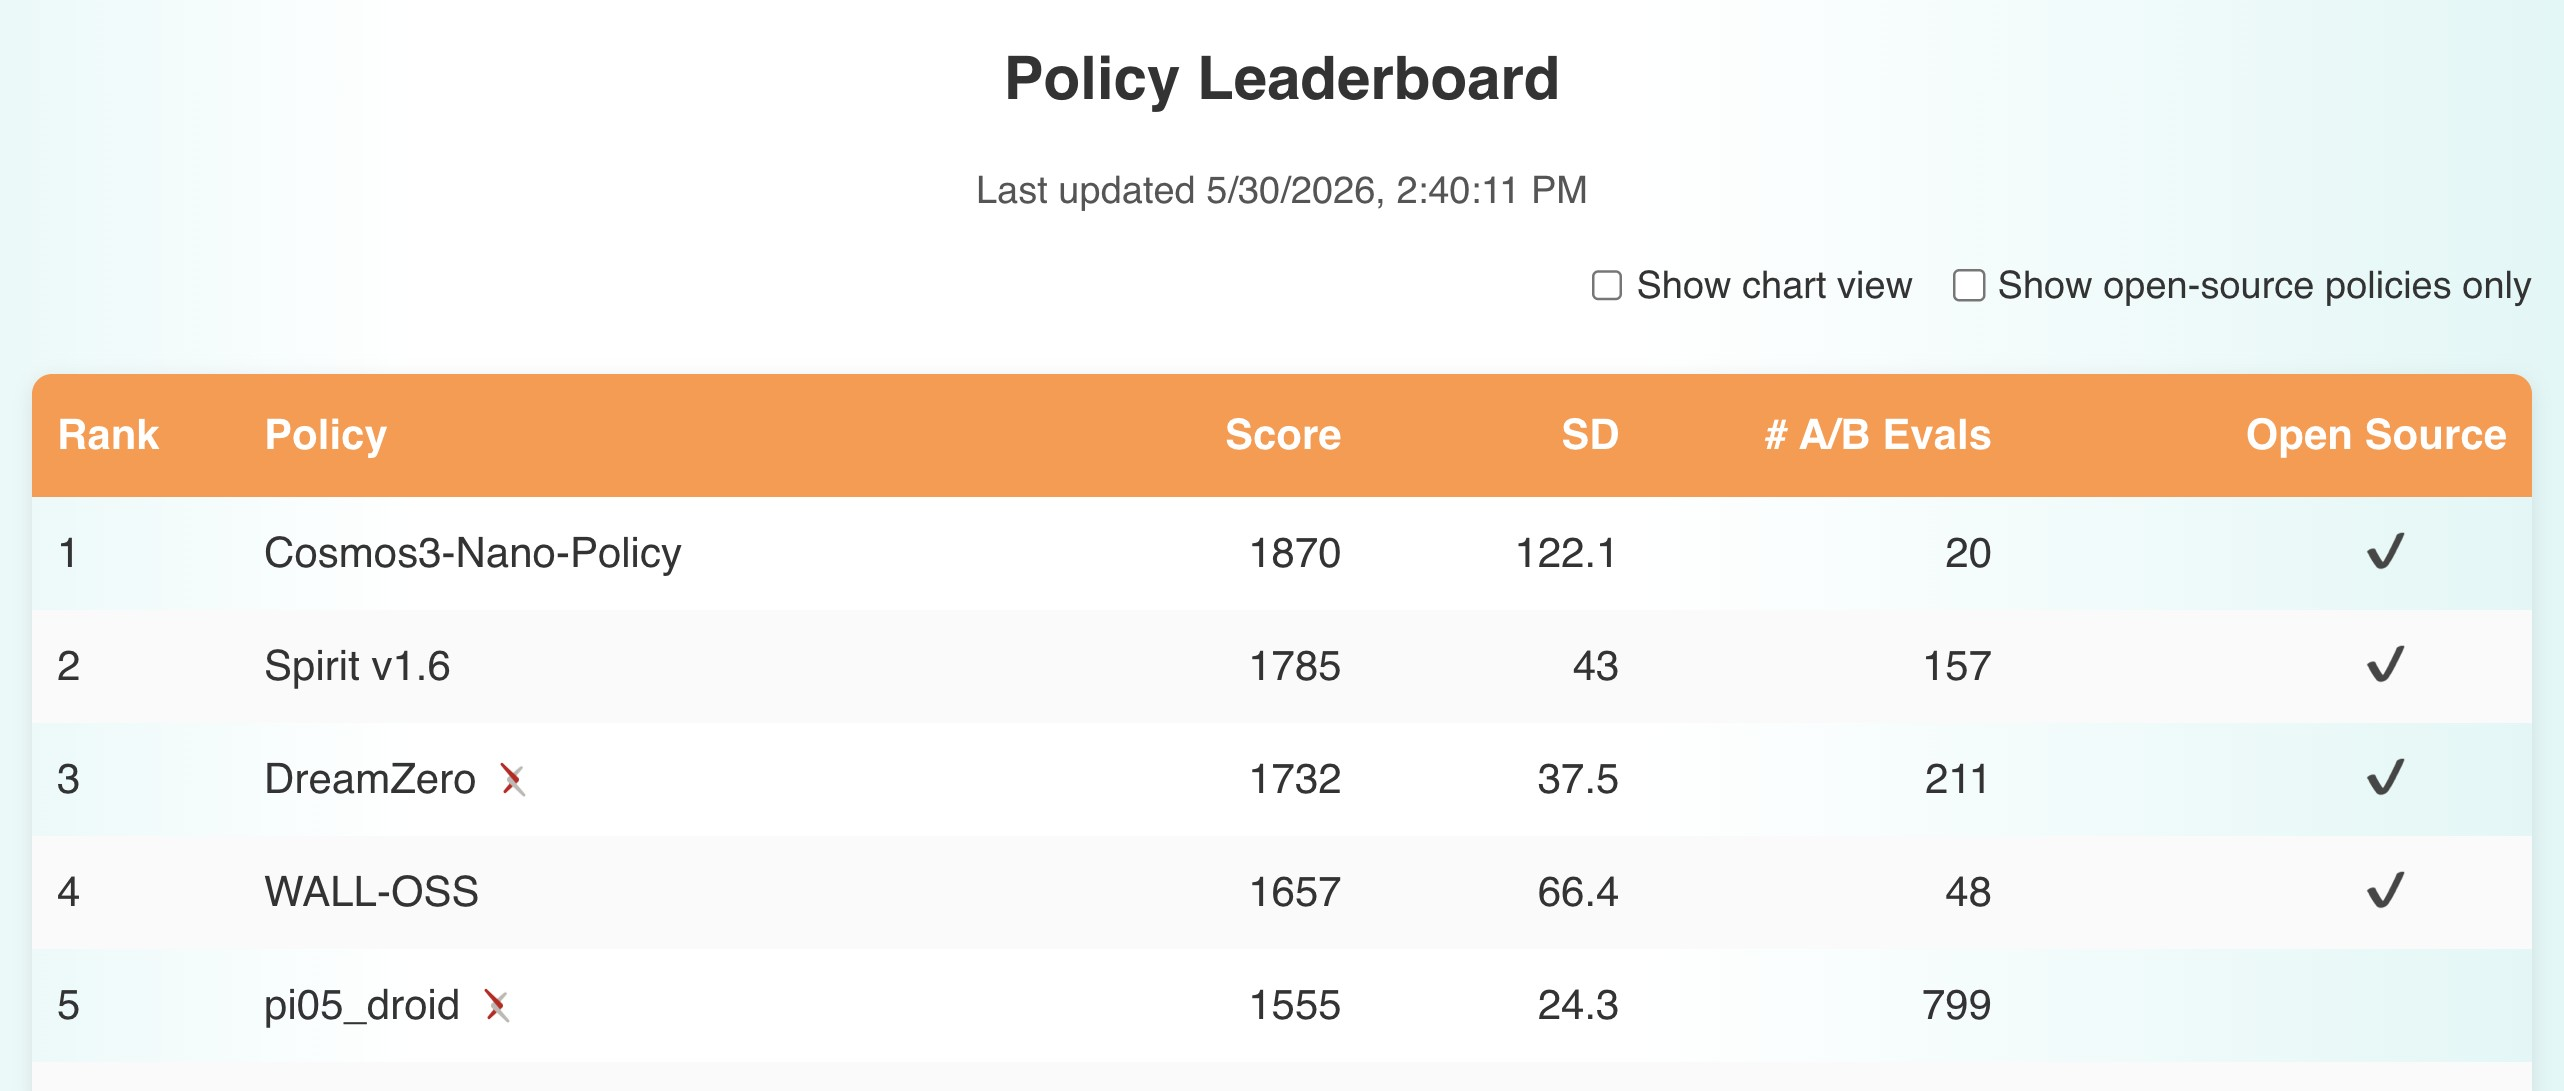
\includegraphics[width=0.85\linewidth]{figures/results/action/roboarena_leaderboard_final.jpg}
    \vspace{0.5em}
    \caption{\textbf{Cosmos3-Nano-Policy-DROID held the top position on RoboArena.}
    Cosmos3-Nano-Policy-DROID ranked \#1 on the RoboArena real-world benchmark leaderboard
    (Date: 2026-05-30).}
    \label{fig:robotarena_leaderboard}
\end{figure}


\paragraph{Adaptation to new embodiments.}
We evaluate whether \textit{MT-init} enables Cosmos3-Nano to adapt more quickly to an unseen embodiment and environment.
We use the LIBERO-10 environment~\citep{liu2023libero} with multi-view observations from a third-person camera and a wrist camera.
We report progress across post-training iterations by running 50 trials per validation task, giving 500 rollouts per checkpoint.

As shown in \cref{tab:libero_posttraining_success_rate}, post-training rapidly improves closed-loop manipulation success rate for both initializations, but \textit{MT-init} has a clear advantage early in post-training.
At 500 iterations, the Cosmos3-Nano \textit{MT-init} reaches 24.6\% success, while the Cosmos3-Nano \textit{PT-init} remains at 0.0\%.
By 2000 iterations, the Cosmos3-Nano \textit{MT-init} can achieve a 97.4\% success rate.
These results show that \textit{MT-init} enables faster adaptation to new embodiments and environments.

\begin{table}[H]
    \centering
    \small
    \caption{
        \textbf{Fast adaptation to a new embodiment using LIBERO-10.} Closed-loop success rates for \textbf{Cosmos3-Nano} from \textit{MT-init} and \textit{PT-init}, evaluated with 500 rollouts per checkpoint. The results show that \textit{MT-init} adapts faster than \textit{PT-init}.
    }
    \label{tab:libero_posttraining_success_rate}
    \begin{tabular}{@{}lrrrr@{}}
        \toprule
        \multirow{2}{*}{\textbf{Model}} & \multicolumn{4}{c}{\textbf{Iteration}} \\
        \cmidrule(lr){2-5}
            & \textbf{500} & \textbf{1000} & \textbf{1500} & \textbf{2000} \\
        \midrule
        \textbf{Cosmos3-Nano} (\textit{MT-init}) & 24.6\% & 91.4\% & 95.8\% & \textbf{97.4\%} \\
        \textbf{Cosmos3-Nano} (\textit{PT-init}) & 0.0\% & 73.8\% & 93.4\% & 95.2\% \\
        \bottomrule
    \end{tabular}
\end{table}


\paragraph{Action data synergy.}
\label{app:action_data_synergy}
Choosing which action domains to train together is a practical mixture-design problem: an added domain can provide a useful visual-action prior, but it can also dilute supervision for the target domain.
Inspired by recent work on language-domain transfer~\citep{longpre2026atlas}, which measures how training on one language benefits or interferes with another, we build analogous transfer maps for action mid-training across ego-motion domains (Camera Motion, Autonomous Vehicle), robot manipulation domains (Google Robot, WidowX-250, Franka Panda Single, Franka Panda Dual, AgiBot), and human egocentric motion (Egocentric).
The quantitative synergy matrices are summarized in~\Cref{fig:action_synergy_av_camera_robots} and~\Cref{fig:action_synergy_agibot}.
We report PSNR for FD and MSE for ID.
For policy mode, we report the minimum PSNR and MSE across 4 rollouts because the rollout distribution is multimodal.
In each synergy matrix, an off-diagonal cell uses a 50/50 mixture of the row and column domains for 4{,}000 iterations, while a diagonal cell is the corresponding single-domain baseline at 2{,}000 iterations.
This setup matches the per-domain training budget between single-domain and paired runs.
Each row fixes the evaluation domain, and columns vary the single-domain or paired training setting.
Positive deltas indicate cross-domain transfer, while negative deltas indicate interference.

We summarize our key findings below:

\begin{figure}[t]
    \centering
    \resizebox{\linewidth}{!}{%
        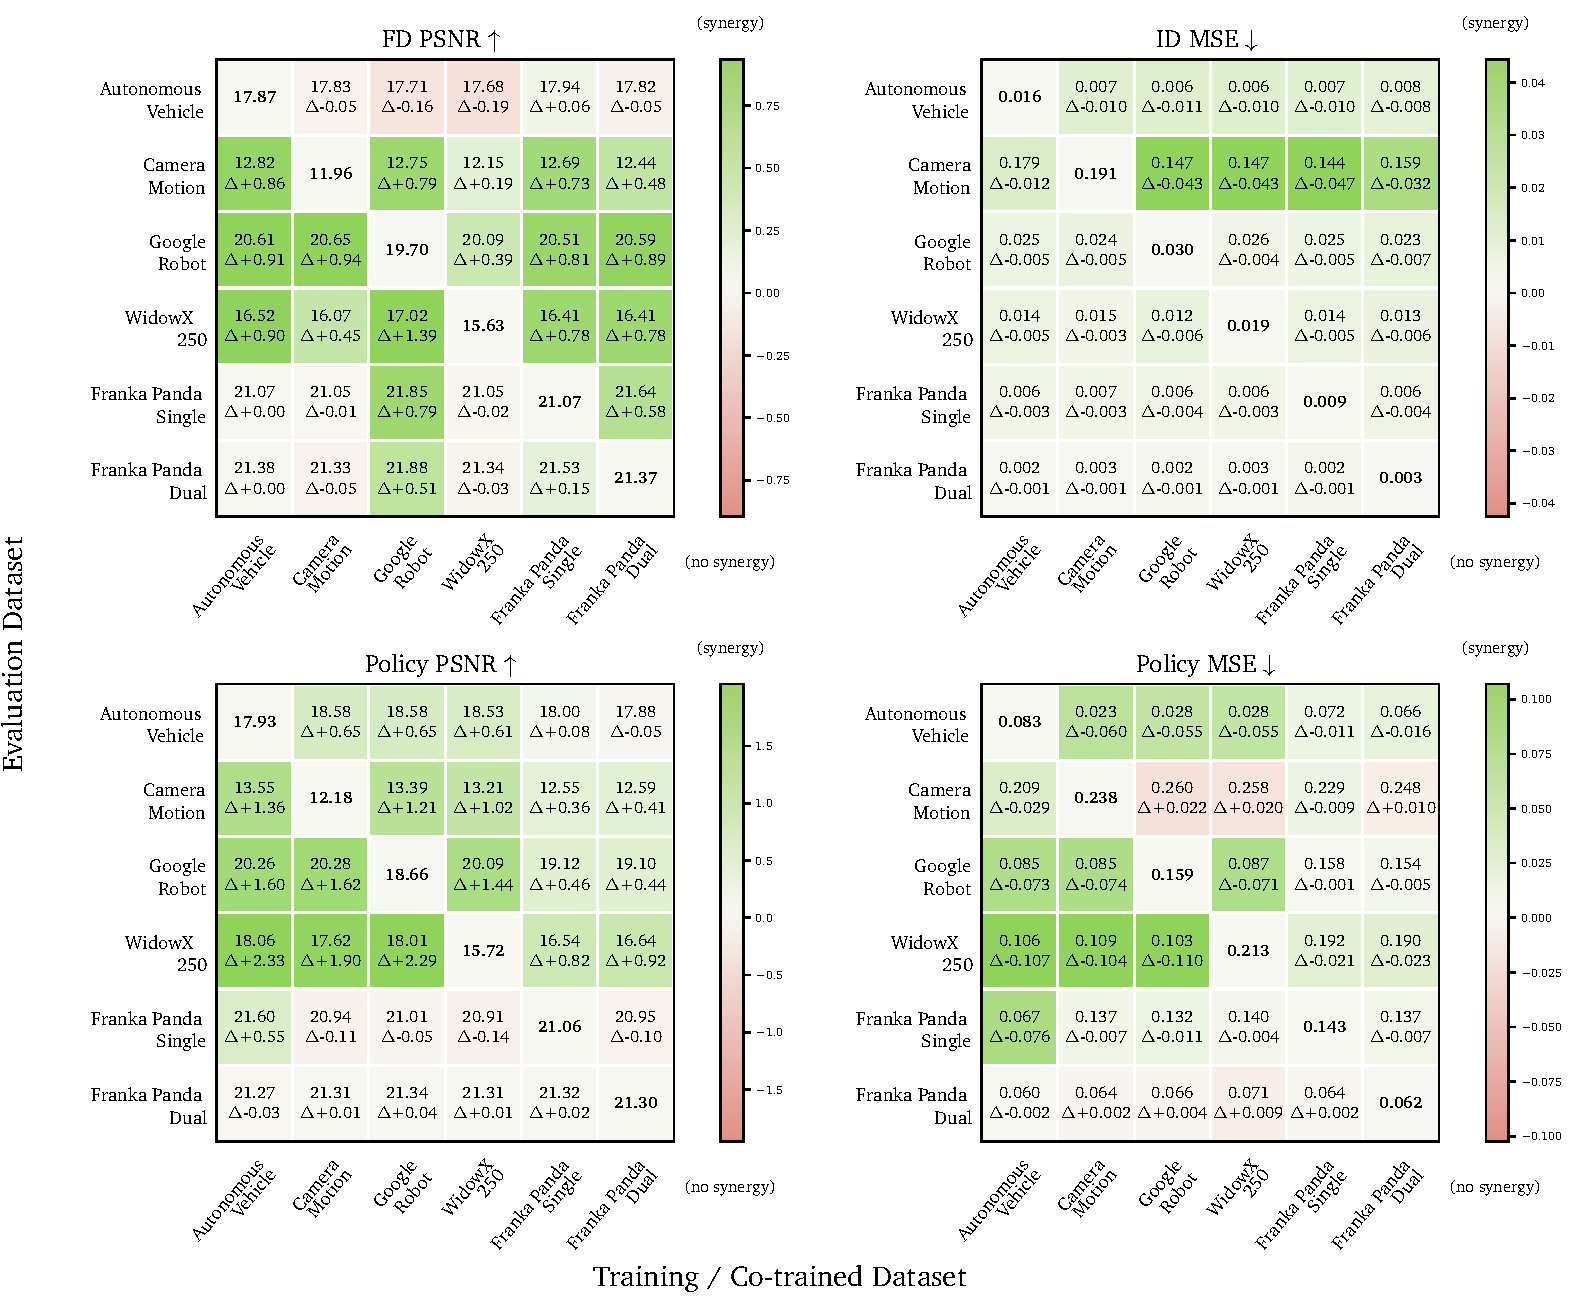
\includegraphics{figures/results/action/synergy/synergy_av_camera_robots_tikz.pdf}%
    }
    \caption{\textbf{Synergy study across ego-motion and robot manipulation domains.}
    Rows denote evaluation domains; columns denote the added co-training domain.
    Diagonal cells are single-domain baselines, while off-diagonal cells use a 50/50 row--column mixture with matched row-domain training exposure.
    Each cell reports the score and delta from the row diagonal.
    Green indicates positive transfer, with signs adjusted so that higher PSNR ($\uparrow$) and lower MSE ($\downarrow$) are both better.}

    \label{fig:action_synergy_av_camera_robots}
\end{figure}


\begin{itemize}[leftmargin=*]
    \item \textit{Camera motion benefits from broad action co-training.}
    \Cref{fig:action_synergy_av_camera_robots} shows that camera motion, one of the lower-performing domains, benefits from several co-training partners rather than only from another ego-motion source.
    AV data improves camera FD PSNR from 11.96 to 12.82 (+0.86), while robot domains also provide positive FD gains, including Google Robot (+0.79), Franka Panda Single (+0.73), and Franka Panda Dual (+0.48).
    ID MSE also improves for every shown co-training partner in the row.
    This suggests that camera-motion learning benefits from general action-conditioned visual priors, such as object persistence, scene geometry, and motion-correspondence cues, even when the added domain has a different embodiment.

    \item \textit{Robot manipulation domains share early-training priors.}
    The robot-domain panels in \Cref{fig:action_synergy_av_camera_robots} show broad early transfer among manipulation datasets, especially for domains with lower-performing single-domain baselines or more heterogeneous data.
    WidowX-250 benefits strongly from Google Robot, gaining +1.39 FD PSNR and +2.29 policy PSNR, with matching improvements in ID and policy MSE.
    Google Robot also gains from several robot co-training partners, with FD PSNR improvements up to +0.89 and policy PSNR improvements up to +1.44.
    By contrast, the Franka Panda single-arm and dual-arm entries in this synergy study correspond to small RoboMIND Franka subsets~\citep{wu2024robomind}, with only 23 and 4 hours of data, respectively. Compared with the much larger action-data sources summarized in~\Cref{fig:action_data_distribution}, these small target domains saturate quickly under single-domain training, so adding larger co-training domains yields smaller or mixed gains on their own evaluations. However, they still provide useful transfer to other domains when used as co-trained sources.

    \item \textit{Human egocentric motion helps robot adaptation.}
    \Cref{fig:action_synergy_agibot_handpose} shows modest but consistent transfer between egocentric motion and AgiBot.
    Egocentric data improves AgiBot FD PSNR from 23.07 to 23.20 (+0.13), while AgiBot slightly improves egocentric FD PSNR from 15.13 to 15.16 (+0.03).
    The warmup curve in \Cref{fig:action_synergy_agibot_curve} further tests this transfer as an initialization effect: we first warm up the base PT-init checkpoint on egocentric motion and then adapt it to AgiBot, comparing against direct AgiBot adaptation from the same PT-init checkpoint.
    Starting from the egocentric-warmed checkpoint improves AgiBot FD PSNR at every measured step, with gains of +0.94 at 5K and roughly +1.3--1.6 later in training.
    Together, these results suggest that egocentric human action data provides a useful manipulation prior for robot adaptation, while domain-aware sampling or specialization remains important as training progresses.
\end{itemize}

\begin{figure}[t]
    \centering
    \captionsetup[subfigure]{font=small,skip=3pt,justification=centering,singlelinecheck=false}

    \begin{subfigure}[t]{0.43\linewidth}
        \centering
        \resizebox{\linewidth}{!}{%
            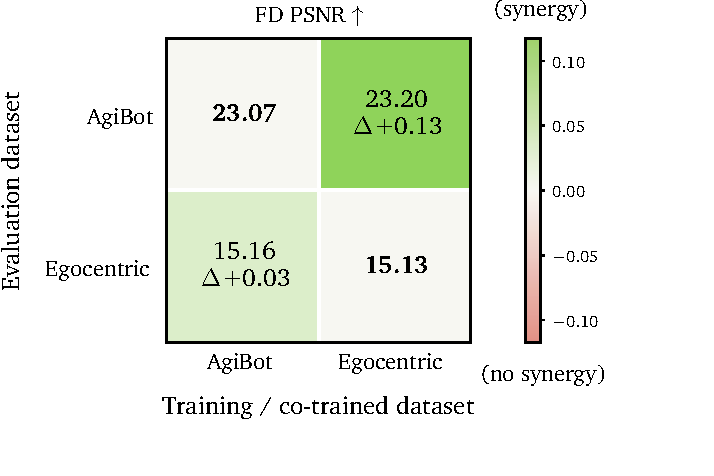
\includegraphics{figures/results/action/synergy/synergy_agibot_handpose_tikz.pdf}%
        }
        \caption{Synergy between AgiBot and Egocentric motion.}
        \label{fig:action_synergy_agibot_handpose}
    \end{subfigure}
    \hfill
    \begin{subfigure}[t]{0.53\linewidth}
        \centering
        \resizebox{\linewidth}{!}{%
            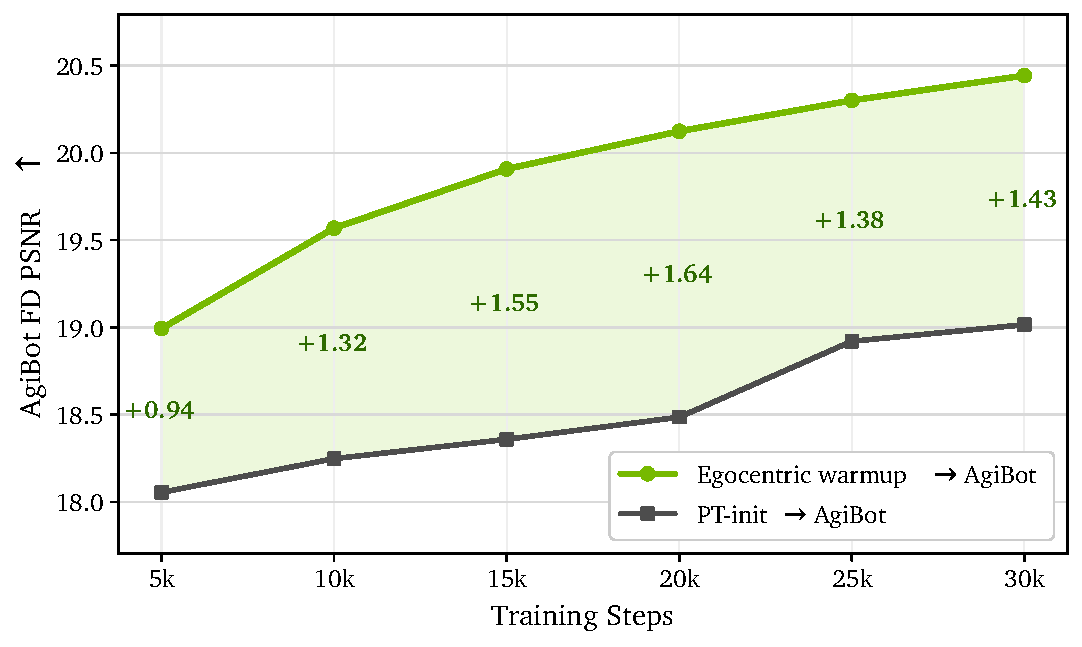
\includegraphics{figures/results/action/synergy/agibot_handpose_curve_tikz.pdf}%
        }
        \caption{AgiBot benefits from Egocentric warmup.}
        \label{fig:action_synergy_agibot_curve}
    \end{subfigure}

    \caption{\textbf{Egocentric motion as a robot-adaptation prior.}
    (a) The matrix measures pairwise transfer between AgiBot robot manipulation and Egocentric motion. (b)
    The curve compares AgiBot adaptation from an Egocentric-warmed checkpoint against direct adaptation from the \textit{PT-init} checkpoint.}
    \label{fig:action_synergy_agibot}
\end{figure}



\paragraph{Conclusion.}
\label{sec:action_exp_summary}
We show that Cosmos 3 is a strong action foundation model across diverse domains, embodiments, and inference modes.
A single foundation model can be adapted to camera-controlled video generation, autonomous-vehicle inverse dynamics, egocentric hand forward dynamics, robot forward dynamics, and robot policy learning, while remaining competitive with or stronger than specialized domain baselines.
The comparison between \textit{PT-init} and \textit{MT-init} further shows that unified action mid-training does more than improve isolated domains: it produces a reusable action-domain prior that accelerates convergence across downstream settings, including adaptation to a new embodiment and environment.
This is especially notable because the evaluated domains differ substantially in embodiment and supervision format, ranging from camera and vehicle motion to articulated human hands and robot end-effectors.
The synergy study provides evidence that action domains share transferable structure: co-training across ego-motion, robot manipulation, and egocentric motion can improve early adaptation, particularly for domains with weaker single-domain baselines.
The additional action-specific ablations in Appendix~\ref{app:pusht_fd_id_policy_synergy} and \ref{app:robolab_video_action_consistency} reinforce the same conclusion: FD, ID, and policy objectives share useful structure under joint training, and videos predicted alongside policy actions remain aligned with simulator rollouts driven by those same actions.
Overall, these findings support Cosmos 3 as a general-purpose world-action foundation model that can be efficiently specialized to a broad range of action generation and control tasks.
